\documentclass[]{article}
\usepackage{lmodern}
\usepackage{amssymb,amsmath}
\usepackage{ifxetex,ifluatex}
\usepackage{fixltx2e} % provides \textsubscript
\ifnum 0\ifxetex 1\fi\ifluatex 1\fi=0 % if pdftex
  \usepackage[T1]{fontenc}
  \usepackage[utf8]{inputenc}
\else % if luatex or xelatex
  \ifxetex
    \usepackage{mathspec}
  \else
    \usepackage{fontspec}
  \fi
  \defaultfontfeatures{Ligatures=TeX,Scale=MatchLowercase}
\fi
% use upquote if available, for straight quotes in verbatim environments
\IfFileExists{upquote.sty}{\usepackage{upquote}}{}
% use microtype if available
\IfFileExists{microtype.sty}{%
\usepackage{microtype}
\UseMicrotypeSet[protrusion]{basicmath} % disable protrusion for tt fonts
}{}
\usepackage[margin=1in]{geometry}
\usepackage{hyperref}
\hypersetup{unicode=true,
            pdftitle={Escalamiento multidimensional},
            pdfauthor={Dra. Rocío Maehara},
            pdfborder={0 0 0},
            breaklinks=true}
\urlstyle{same}  % don't use monospace font for urls
\usepackage{graphicx,grffile}
\makeatletter
\def\maxwidth{\ifdim\Gin@nat@width>\linewidth\linewidth\else\Gin@nat@width\fi}
\def\maxheight{\ifdim\Gin@nat@height>\textheight\textheight\else\Gin@nat@height\fi}
\makeatother
% Scale images if necessary, so that they will not overflow the page
% margins by default, and it is still possible to overwrite the defaults
% using explicit options in \includegraphics[width, height, ...]{}
\setkeys{Gin}{width=\maxwidth,height=\maxheight,keepaspectratio}
\IfFileExists{parskip.sty}{%
\usepackage{parskip}
}{% else
\setlength{\parindent}{0pt}
\setlength{\parskip}{6pt plus 2pt minus 1pt}
}
\setlength{\emergencystretch}{3em}  % prevent overfull lines
\providecommand{\tightlist}{%
  \setlength{\itemsep}{0pt}\setlength{\parskip}{0pt}}
\setcounter{secnumdepth}{0}
% Redefines (sub)paragraphs to behave more like sections
\ifx\paragraph\undefined\else
\let\oldparagraph\paragraph
\renewcommand{\paragraph}[1]{\oldparagraph{#1}\mbox{}}
\fi
\ifx\subparagraph\undefined\else
\let\oldsubparagraph\subparagraph
\renewcommand{\subparagraph}[1]{\oldsubparagraph{#1}\mbox{}}
\fi

%%% Use protect on footnotes to avoid problems with footnotes in titles
\let\rmarkdownfootnote\footnote%
\def\footnote{\protect\rmarkdownfootnote}

%%% Change title format to be more compact
\usepackage{titling}

% Create subtitle command for use in maketitle
\providecommand{\subtitle}[1]{
  \posttitle{
    \begin{center}\large#1\end{center}
    }
}

\setlength{\droptitle}{-2em}

  \title{\textbf{Escalamiento multidimensional}}
    \pretitle{\vspace{\droptitle}\centering\huge}
  \posttitle{\par}
    \author{Dra. Rocío Maehara}
    \preauthor{\centering\large\emph}
  \postauthor{\par}
      \predate{\centering\large\emph}
  \postdate{\par}
    \date{16 de noviembre de 2019}


\begin{document}
\maketitle

\subsection{Introducción}\label{introducciuxf3n}

El análisis de escalamiento multidimensional (MDS) es una { técnica de
reducción de datos } como otras que hemos visto anteriormente: análisis
factorial o análisis de componentes principales, por ejemplo. El {
objetivo principal } del MDS es {representar \(N\) objetos en un espacio
dimensional reducido (\(q\) dimensiones, siendo \(q < N\)) }, de tal
forma que la { distorsión causada por la reducción de la dimensionalidad
sea la menor posible }, es decir, que las distancias entre los objetos
representados en el espacio \(q\) dimensional sean lo más parecidas
posible a las distancias en el espacio \(N\) dimensional.

\subsection{Introducción}\label{introducciuxf3n-1}

Dado que será { difícil que las distancias coincidan}, el objetivo del
MDS es {conseguir que ambas configuraciones dimensionales sean lo más
parecidas posible}, Para ello será necesario construir un {indicador de
esa proximidad } que, como se detallará más adelante, denominaremos
{stress o sstress}.

\subsection{Valoración de la imagen de superficies
comerciales}\label{valoraciuxf3n-de-la-imagen-de-superficies-comerciales}

\hypertarget{left}{}
\begin{verbatim}
datos <- matrix(c(
0.0, 1.0, 2.1, 6.1, 5.2,
1.0, 0.0, 2.4, 6.9, 5.3,
2.1, 2.4, 0.0, 5.1, 4.1,
6.1, 6.9, 5.1, 0.0, 3.1,
5.2, 5.3, 4.1, 3.1,0.0), ncol=5, nrow=5, byrow=T,
dimnames=list(c("X1","X2","X3","X4","X5")))
datos
\end{verbatim}

\begin{verbatim}
##    [,1] [,2] [,3] [,4] [,5]
## X1  0.0  1.0  2.1  6.1  5.2
## X2  1.0  0.0  2.4  6.9  5.3
## X3  2.1  2.4  0.0  5.1  4.1
## X4  6.1  6.9  5.1  0.0  3.1
## X5  5.2  5.3  4.1  3.1  0.0
\end{verbatim}

\hypertarget{right}{}
Supongamos que hemos pedido a {100 consumidores} que valoren la {imagen
que tienen de 5 superficies comerciales}, atendiendo a la similitud con
que las perciben. Para ello se utiliza una {escala de 0 (idénticas) a 7
(totalmente diferentes)}. La siguiente {matriz de disparidades
originales o proximidades} nos muestra las {medias de las puntuaciones}
ofrecidas por los 100 consumidores.

\subsection{Valoración de la imagen de superficies
comerciales}\label{valoraciuxf3n-de-la-imagen-de-superficies-comerciales-1}

\hypertarget{left}{}
\begin{verbatim}
datos <- matrix(c(
0.0, 1.0, 2.1, 6.1, 5.2,
1.0, 0.0, 2.4, 6.9, 5.3,
2.1, 2.4, 0.0, 5.1, 4.1,
6.1, 6.9, 5.1, 0.0, 3.1,
5.2, 5.3, 4.1, 3.1,0.0), ncol=5, nrow=5, byrow=T,
dimnames=list(c("X1","X2","X3","X4","X5")))
datos
\end{verbatim}

\begin{verbatim}
##    [,1] [,2] [,3] [,4] [,5]
## X1  0.0  1.0  2.1  6.1  5.2
## X2  1.0  0.0  2.4  6.9  5.3
## X3  2.1  2.4  0.0  5.1  4.1
## X4  6.1  6.9  5.1  0.0  3.1
## X5  5.2  5.3  4.1  3.1  0.0
\end{verbatim}

\hypertarget{right}{}
Si creamos un {mapa en dos dimensiones} para ilustrar mejor la
percepción de los consumidores, este mapa debería representar como
{puntos cercanos a las superficies \(X_1\) y \(X_2\)} porque la
{disparidad} entre ellas es{ pequeña (1.0)}, tal y como refleja la
matriz. Asimismo, las {superficies \(X_2\) y \(X_4\)} deberían aparecer
representadas muy {distantes} una de la otra, por cuanto su {disparidad}
en la matriz es {elevada (6.9)}.

\subsection{Valoración de la imagen de superficies
comerciales}\label{valoraciuxf3n-de-la-imagen-de-superficies-comerciales-2}

\hypertarget{left}{}
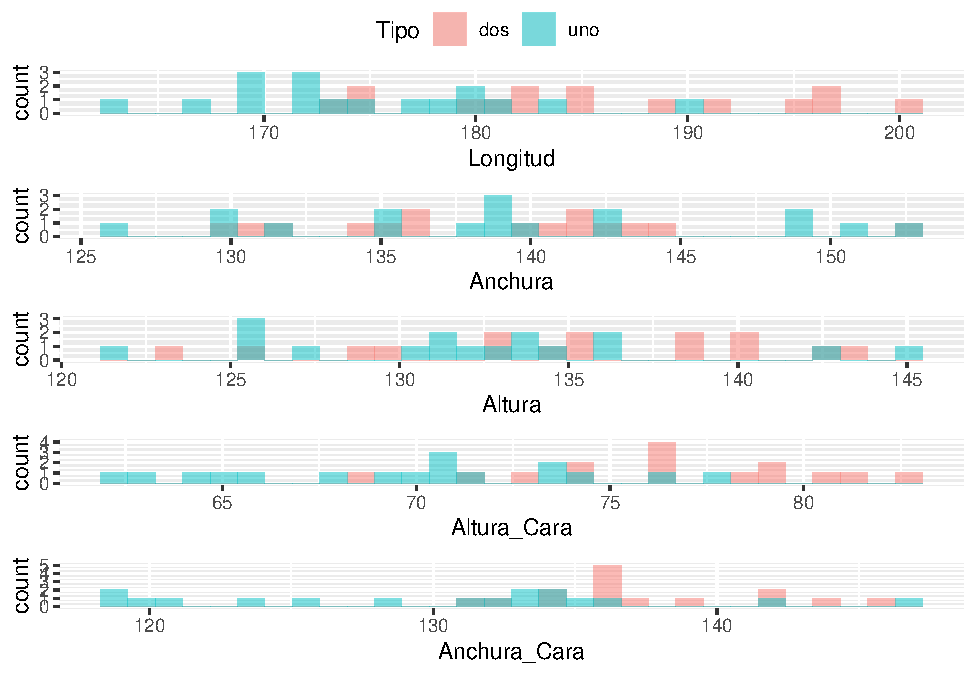
\includegraphics{Clase-4_files/figure-latex/unnamed-chunk-3-1.pdf}

\hypertarget{right}{}
\begin{verbatim}
library(smacof)
fit2 <- mds(delta=datos,ndim=2, type="interval")
plot(fit2, main = "Datos de la imagen de cadenas de electrodomésticos")
\end{verbatim}

Se puede apreciar el {mapa} que se obtiene al {representar las
coordenadas bidimensionales} resultantes de aplicar a la matriz anterior
uno de los algoritmos que existen para efectuar un MDS, el implementado
en \texttt{mds(smacof)}. Puede comprobarse como se constata la {cercanía
de \(X_1\) y \(X_2\)} y la {lejanía de \(X_2\) y \(X_4\)} que
esperábamos.

\subsection{Desarrollo formal de la técnica
MSD}\label{desarrollo-formal-de-la-tuxe9cnica-msd}

Con el ejemplo de las superficies comerciales expuesto con anterioridad.
Si {partimos de \(N\) objetos (superficies comerciales)}, tendremos
entonces {\(M=N(N—1)/2\) disparidades originales} entre pares de objetos
(10 en nuestro ejemplo). Asumiendo que no haya empates (los distintos
algoritmos resuelven los empates de distintos modos), las {disparidades}
pueden escribirse en un {orden estrictamente ascendente}:
\[s_{i_1k_1}<s_{i_2k_2}<\ldots<s_{i_Mk_M}\] donde {\(s_{i_1k_1}\)} es la
{menor de las disparidades}. El subíndice \(i_1k_1\) indica el {par de
objetos} que son {más parecidos}.

\subsection{El algoritmo básico del
MDS}\label{el-algoritmo-buxe1sico-del-mds}

En nuestro ejemplo esta ordenación sería la siguiente:
\[1.0< 2.1< 2.4< 3.1< 4.1< 5.1< 5.2< 5.3< 6.1< 6.9\]
\[s_{12}<s_{13}<s_{23}<s_{45}<s_{35}<s_{34}<s_{15}<s_{25}<s_{14}<s_{24}\]

Nuestro {objetivo} es encontrar una {nueva configuración \(q\)
dimensional} de los \(N\) objetos (2 dimensiones y 5 objetos en el
ejemplo), de tal forma que las {distancias calculadas entre ellos en ese
espacio \(q\) dimensional mantengan la ordenación anterior}. En el caso
ideal de que se {mantuviera el orden y las proporciones entre
disparidades y distancias}, el {gráfico de dispersión} entre ambas se
representaría mediante una {línea recta}.

\subsection{El algoritmo básico del
MDS}\label{el-algoritmo-buxe1sico-del-mds-1}

\hypertarget{left}{}
\begin{verbatim}
# Solución bidimensional
fit2$conf
\end{verbatim}

\begin{verbatim}
##            D1          D2
## X1 -0.5504010  0.01970998
## X2 -0.6430815 -0.04506942
## X3 -0.2233691  0.14315764
## X4  0.8854840  0.20160756
## X5  0.5313676 -0.31940576
\end{verbatim}

\hypertarget{right}{}
En el MDS se van {ensayando distintas configuraciones \(q\)
dimensionales} hasta que las {distancias en ese espacio y las
disparidades originales guarden una relación lo más próxima posible a
esta recta ideal}. El código muestra la {solución bidimensional final}
resultante de la aplicación del MDS a los datos de nuestro ejemplo. En
este cuadro aparecen las {coordenadas de cada objeto (superficie
comercial) en ese espacio bidimensional}.

\subsection{El algoritmo básico del
MDS}\label{el-algoritmo-buxe1sico-del-mds-2}

\hypertarget{left}{}
\begin{verbatim}
#Distancias entre las configuraciones
print(fit2$confdist)
\end{verbatim}

\begin{verbatim}
##           X1        X2        X3        X4
## X2 0.1130754                              
## X3 0.3495557 0.4599869                    
## X4 1.4473605 1.5483417 1.1103925          
## X5 1.1336767 1.2060644 0.8852075 0.6299629
\end{verbatim}

\begin{verbatim}
##            D1          D2
## X1 -0.5504010  0.01970998
## X2 -0.6430815 -0.04506942
## X3 -0.2233691  0.14315764
## X4  0.8854840  0.20160756
## X5  0.5313676 -0.31940576
\end{verbatim}

\hypertarget{right}{}
A partir de esas {coordenadas} es sencillo derivar la {matriz de
distancia entre los distintos objetos}. Así, tomando {distancias
euclídeas}, la distancia entre, por ejemplo, X1 y X2 tomaría el valor:
\[d(X_1,X_2)=\sqrt{(-0.5504-(-0.6431))^2+(0.0197-(-0.0451))^2}=0.1131\]
Repitiendo los cálculos para todos los objetos (estímulos), obtendríamos
la {matriz de distancias \(\textbf{D}\) entre las configuraciones}
mostrada en el código.

\subsection{El algoritmo básico del
MDS}\label{el-algoritmo-buxe1sico-del-mds-3}

\hypertarget{left}{}
\begin{verbatim}
# Matriz de disparidades
print(fit2$dhat)
\end{verbatim}

\begin{verbatim}
##           X1        X2        X3        X4
## X2 0.1001109                              
## X3 0.3773818 0.4530011                    
## X4 1.3856397 1.5872913 1.1335752          
## X5 1.1587817 1.1839881 0.8815108 0.6294463
\end{verbatim}

\hypertarget{right}{}
En el algoritmo del MDS se obtiene, como hemos señalado, una
{transformación monótona de la matriz de distancias originales en el
espacio \(N\) dimensional} y es respecto a esa {transformación (matriz
de disparidades \(\Delta\))} obtenida en {cada iteración} con la que {se
va comparando la matriz \(\textbf{D}\)}. El código muestra la {solución
final bidimensional} alcanzada en la {última iteración proporciona la
matriz de disparidades \(\Delta\)}.

\subsection{El algoritmo básico del
MDS}\label{el-algoritmo-buxe1sico-del-mds-4}

\hypertarget{left}{}
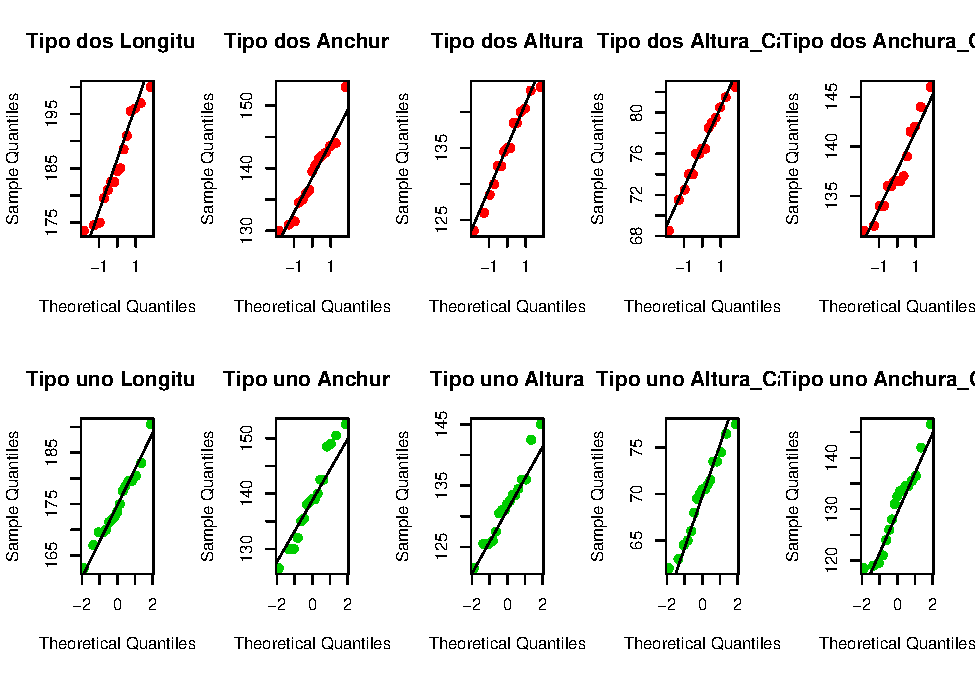
\includegraphics{Clase-4_files/figure-latex/unnamed-chunk-8-1.pdf}

\hypertarget{right}{}
\begin{verbatim}
plot(fit2,plot.type="Shepard",plot.dim=c(1,2),sphere=TRUE,bubscale=0.1,col=1,
label.conf=list(label=TRUE,pos=3,col=1,cex=0.8),
shepard.x=NULL,identify=FALSE,
type="p",pch=20,asp=1,col.hist=NULL)
\end{verbatim}

Así pues, la {matriz de disparidades \(\Delta\)} es simplemente una
{transformación monótona de la matriz de distancias originales
\(\textbf{S}\)}. Esto se puede comprobar representando, simplemente, en
un {gráfico de dispersión las distancias que aparecen en ambas}. Este
gráfico es conocido como {diagrama de Shepard}, donde los {puntos sobre
la diagonal} muestran la {transformación monótona} y los {puntos grises}
muestran las {discrepancias que se producen}, que serán un {indicador de
la bondad del ajuste} del modelo que veremos posteriormente.

\subsection{El algoritmo básico del
MDS}\label{el-algoritmo-buxe1sico-del-mds-5}

El algoritmo usado en la técnica MDS ensaya distintas configuraciones
bidimensionales hasta dar con aquella que {reduce en mayor grado las
diferencias entre las matrices de distancias \(\textbf{D}\) y
disparidades \(\Delta\)}. Para ello necesitamos una función objetivo que
se minimizará en cada iteración. Kruskal (1964a) propuso la siguiente
función, que denominó stress:
\[Stress=\sqrt{\frac{\sum_{i \neq j} (d_{ij}-\delta_{ij})^2}{\sum_{i \neq j} d^2_{ij}}}\]
donde {\(d_{ij}\)} son los {elementos de la matriz de distancias}
resultante de la solución \(q\) dimensional en la interación que se esté
realizando y {\(\delta_{ij}\)} son los {elementos de la matriz de
disparidades} que, recordemos, no son sino una transformación monótona
de los elementos de la matriz de disparidades originales entre los
distintos objetos (estímulos).

\subsection{El algoritmo básico del
MDS}\label{el-algoritmo-buxe1sico-del-mds-6}

\hypertarget{left}{}
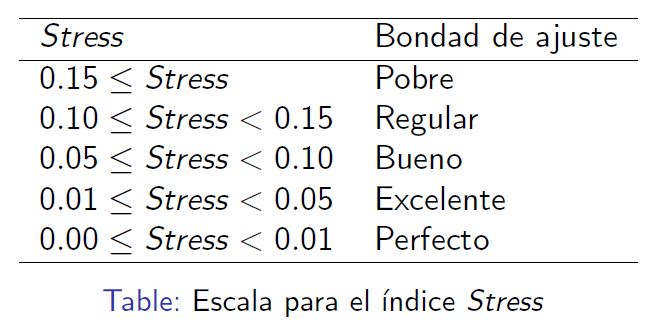
\includegraphics[width=1\linewidth]{images/stress}

\hypertarget{right}{}
En síntesis, el {stress} no es sino un {indicador} de {cuánto difieren
en promedio} la {matriz con las distancias de la solución dimensional
reducida} respecto a la {matriz con las disparidades originales}. El
cuadrado del numerador pretende, únicamente, que no se compensen
diferencias positivas con negativas. El valor del {stress} deberá ser
{tan pequeño como sea posible} y, en todo caso, reducirse en cada
iteración. De no ser así, el algoritmo se detendrá.

\subsection{El algoritmo básico del
MDS}\label{el-algoritmo-buxe1sico-del-mds-7}

Una {segunda medida} de las {discrepancias entre las matrices de
disparidades y distancias} y, por ello, de calidad de la representación
lograda por el MDS, es el estadístico denominado s-stress que fue
propuesto por Takane et al. (1977) autores del algoritmo ALSCAL y que,
por ello, es la función que se minimiza en ese algoritmo:
\[S-stress=\sqrt{\frac{\sum_{i \neq j} (d_{ij}-\delta_{ij})^2}{\sum_{i \neq j} d^4_{ij}}}\]
El valor del {s-stress} está siempre {comprendido entre 0 y 1} y
cualquier {valor inferior a 0.1} indica que la {solución obtenida} es
una {buena representación} de los objetos de la solución \(N\)
dimensional inicial.

\subsection{El algoritmo básico del
MDS}\label{el-algoritmo-buxe1sico-del-mds-8}

\hypertarget{left}{}
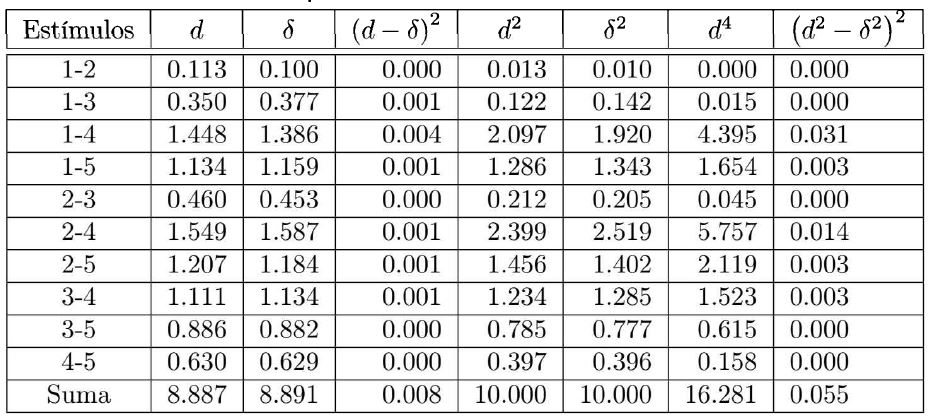
\includegraphics[width=1\linewidth]{images/estimulos}

\hypertarget{right}{}
 Matriz de disparidades \(\Delta\)

\begin{verbatim}
print(fit2$dhat)
\end{verbatim}

\begin{verbatim}
##           X1        X2        X3        X4
## X2 0.1001109                              
## X3 0.3773818 0.4530011                    
## X4 1.3856397 1.5872913 1.1335752          
## X5 1.1587817 1.1839881 0.8815108 0.6294463
\end{verbatim}

Distancias entre configuraciones \(\textbf{D}\)

\begin{verbatim}
print(fit2$confdist)
\end{verbatim}

\begin{verbatim}
##           X1        X2        X3        X4
## X2 0.1130754                              
## X3 0.3495557 0.4599869                    
## X4 1.4473605 1.5483417 1.1103925          
## X5 1.1336767 1.2060644 0.8852075 0.6299629
\end{verbatim}

\subsection{El algoritmo básico del
MDS}\label{el-algoritmo-buxe1sico-del-mds-9}

\hypertarget{left}{}
Stress

\begin{verbatim}
print(fit2$stress)
\end{verbatim}

\begin{verbatim}
## [1] 0.02826073
\end{verbatim}

Stress por punto

\begin{verbatim}
print(fit2$spp)
\end{verbatim}

\begin{verbatim}
##        X1        X2        X3        X4        X5 
## 33.694099 13.906328  8.603052 36.712519  7.084002
\end{verbatim}

\hypertarget{right}{}
La salida de smacof proporciona el valor final del stress. Dado que este
paquete no optimiza no calcula el s-stress. Se comprueba que el stress
0.0282 obtenido alcanza el valor de ``excelente''. El paquete smacof
permite también analizar la contribución de cada punto representado al
stress, es decir, del total del desajuste, qué parte es debida a una
mala representación de un punto determinado. En el caso del ejemplo,
vemos que el punto peor representado sería el \(X_4\) que supone el
36,7\% del total del stress.

\subsection{El algoritmo básico del
MDS}\label{el-algoritmo-buxe1sico-del-mds-10}

\hypertarget{left}{}
\begin{verbatim}
plot(fit2, plot.type = "bubbleplot")
\end{verbatim}

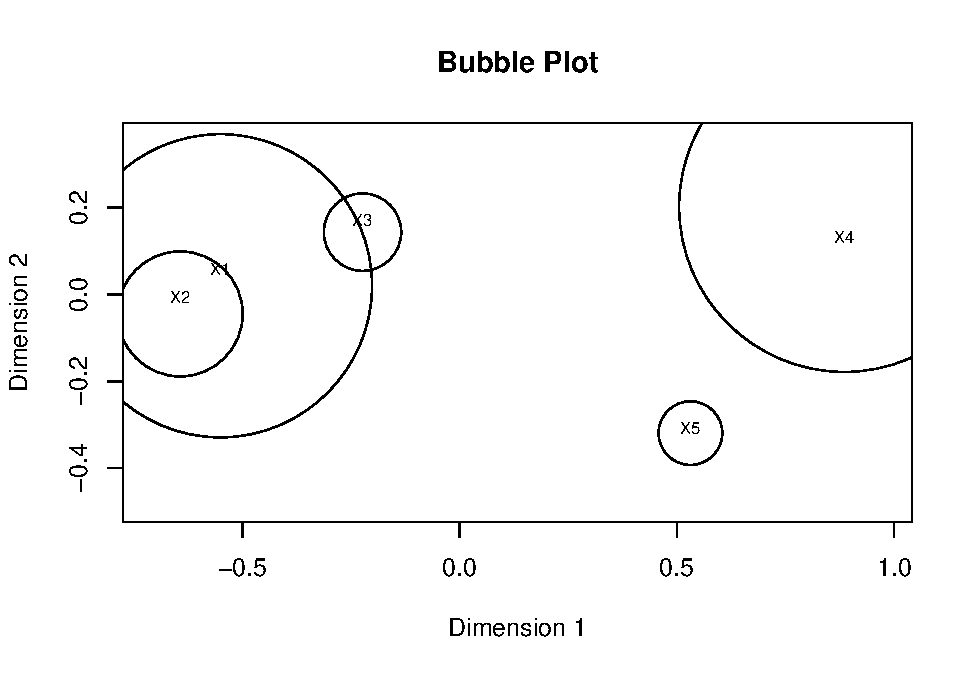
\includegraphics{Clase-4_files/figure-latex/unnamed-chunk-13-1.pdf}

\begin{verbatim}
plot(fit2, plot.type = "stressplot")
\end{verbatim}

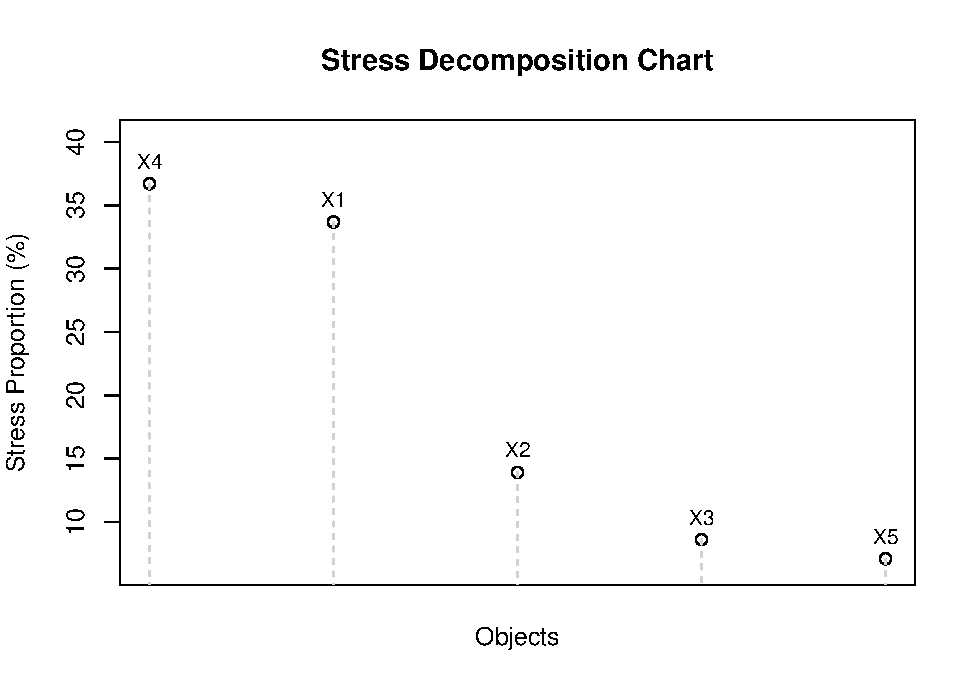
\includegraphics{Clase-4_files/figure-latex/unnamed-chunk-14-1.pdf}

\subsection{El algoritmo básico del
MDS}\label{el-algoritmo-buxe1sico-del-mds-11}

\hypertarget{left}{}
\begin{verbatim}
print(1-fit2$rss)
\end{verbatim}

\begin{verbatim}
## [1] 0.9920133
\end{verbatim}

\hypertarget{right}{}
Como ya se indicó, la solución dimensional reducida es una buena
representación de la solución \(N\) dimensional si la ordenación de las
distancias entre los objetos de la primera mantiene la ordenación de las
disparidades originales de la segunda. En el caso ideal, el gráfico de
dispersión que representara distancias y disparidades debería ser una
línea recta.

\subsection{El algoritmo básico del
MDS}\label{el-algoritmo-buxe1sico-del-mds-12}

\hypertarget{left}{}
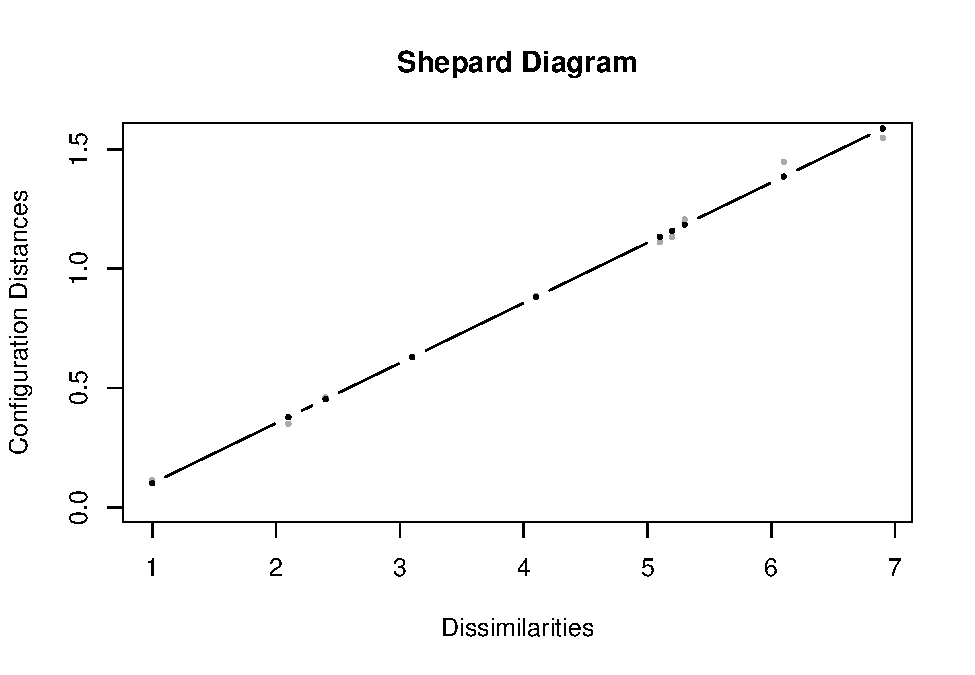
\includegraphics{Clase-4_files/figure-latex/unnamed-chunk-16-1.pdf}

\hypertarget{right}{}
Del análisis del diagrama de Shepard se desprende que la ordenación
lograda con las distancias coincide de manera prácticamente perfecta con
las disparidades. Ahora cabe preguntarse ¿en qué medida se aleja la
relación que se ha representado de la relación ideal? Si efectuáramos
una regresión simple tomando las disparidades como variables
independientes y las distancias como dependientes, el coeficiente de
determinación de esta regresión sería un buen indicador de lo cercano al
ideal de la solución obtenida. Pues bien, ese coeficiente de
determinación es el indicador RSQ que como vimos tiene un valor cercano
a la unidad (0.9920).

\subsection{Recogida de datos para un
escalamiento}\label{recogida-de-datos-para-un-escalamiento}

 El input básico del MDS es, como ya hemos señalado, la similaridad
entre cada par de los \(N\) objetos que se están analizando. A esta
medida, se la suele denominar también proximidad, tal como se ha
apuntado. Estas medidas pueden obtenerse de muy diversas formas. Las dos
más habituales son: - Pedir a los individuos que emitan un juicio de
similaridad entre cada par de estímulos. - Que puntúen en qué grado un
atributo determinado está presente en el estímulo. Al primer tipo de
medidas se las conoce como similaridades directas y al segundo como
similaridades derivadas.

\subsection{Tipos de escalamiento
multidimensional}\label{tipos-de-escalamiento-multidimensional}

 El escalamientos multidimensional no es una técnica, sino un conjunto
de ellas. Los elementos que permiten diferenciarlas son:

\begin{itemize}
\tightlist
\item
  El número de matrices de proximidades.
\item
  La forma de las mismas (cuadradas o rectangulares).
\item
  Si el algoritmo contempla o no ponderaciones. 
\end{itemize}

\subsection{Escalamiento multidimensional
clásico}\label{escalamiento-multidimensional-cluxe1sico}

 Esta formado por una única matriz de proximidades y esta es cuadrada.
Existen dos tipos de esclamiento multidimensional clásico en función de
cómo sean las medidas de similaridad.

\begin{itemize}
\item
  Métrico: Asume que la medidas de similaridad son de intervalo o de
  razón. Este seria el caso, por ejemplo, de una matriz donde los
  estímulos son ciudades, y la medida de proximidad, la distancia en
  kilémetros.
\item
  No métrico: Donde el nivel de medida de la variables es ordinal. 
\end{itemize}

\subsection{Escalamiento multidimensional
clásico}\label{escalamiento-multidimensional-cluxe1sico-1}

 En la función \texttt{mds\{smacof\}} que es la que estima este tipo de
escalamiento, la opción por uno u otro instrumento de medida se elige
con el modificador
\texttt{type=c("ratio","interval","ordinal","mspline")}.

\subsection{Desarrollo educativo de distintas zonas del
mundo}\label{desarrollo-educativo-de-distintas-zonas-del-mundo}

\hypertarget{left}{}
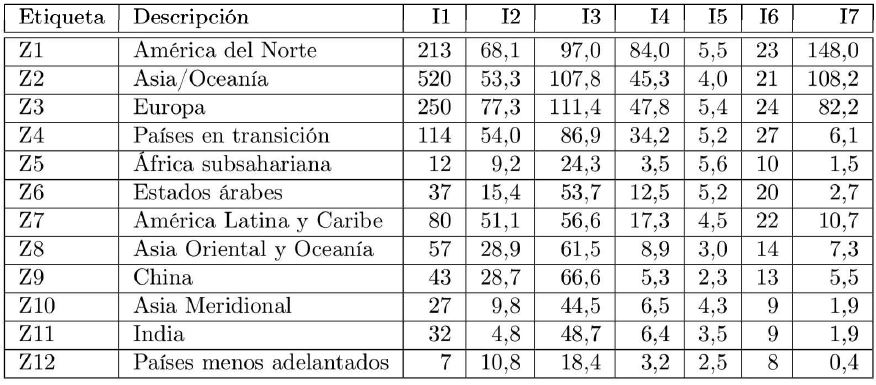
\includegraphics[width=1\linewidth]{images/cuadro}

\hypertarget{right}{}
Supongamos que un investigador en economía de la educación desea saber
cuál es la posición relativa de distintas zonas del mundo respecto al
nivel de desarrollo educativo. En la tabla se recogen los principales
indicadores que este investigador maneja para esta finalidad. Es obvio
que podría recurrirse a un análisis de conglomerados para conseguir un
número de grupos territoriales homogéneos, pero estos grupos estarán
próximos o alejados entre sí. Estas distancias, para el investigador,
son relevantes porque le muestran las diferencias regionales y el camino
que queda por recorrer.

\subsection{Desarrollo educativo de distintas zonas del
mundo}\label{desarrollo-educativo-de-distintas-zonas-del-mundo-1}

\hypertarget{left}{}
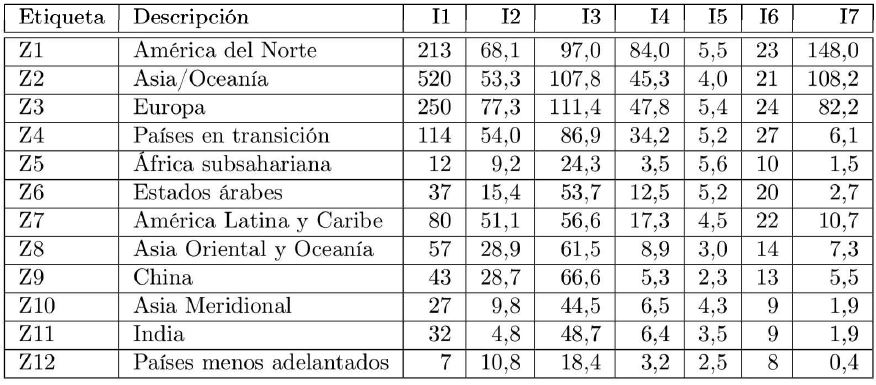
\includegraphics[width=1\linewidth]{images/cuadro}

\hypertarget{right}{}
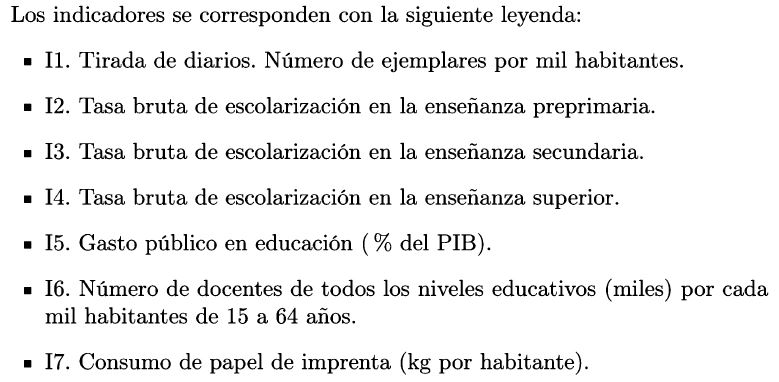
\includegraphics[width=1\linewidth]{images/indi}

\subsection{Desarrollo educativo de distintas zonas del
mundo}\label{desarrollo-educativo-de-distintas-zonas-del-mundo-2}

\hypertarget{left}{}
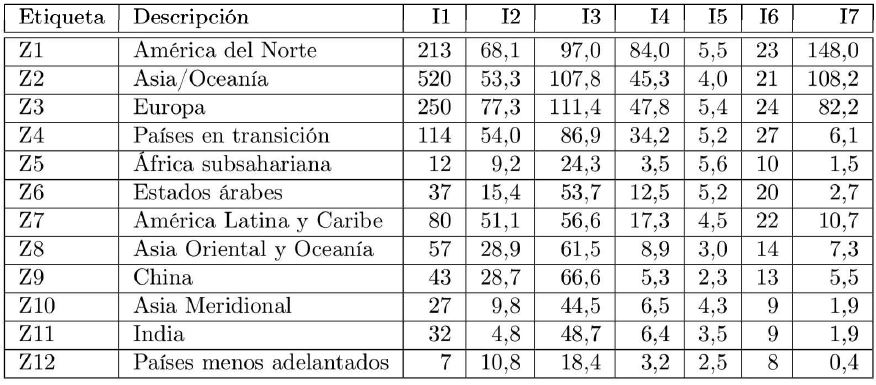
\includegraphics[width=1\linewidth]{images/cuadro}

\hypertarget{right}{}
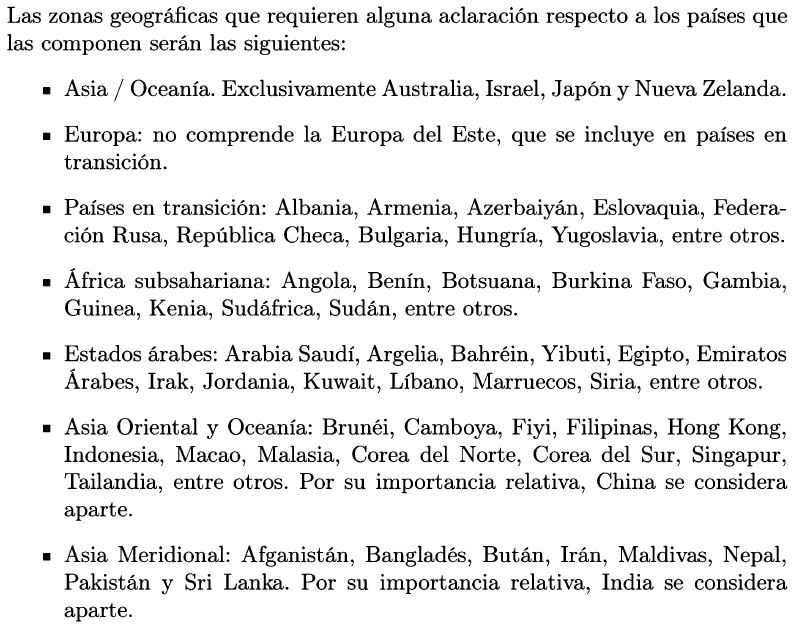
\includegraphics[width=1\linewidth]{images/geogra}

\subsection{Desarrollo educativo de distintas zonas del
mundo}\label{desarrollo-educativo-de-distintas-zonas-del-mundo-3}

\hypertarget{left}{}
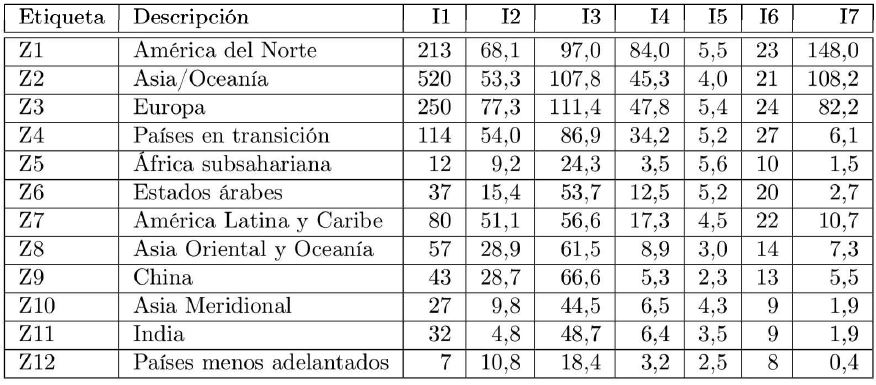
\includegraphics[width=1\linewidth]{images/cuadro}

\hypertarget{right}{}
• Países menos adelantados. Se consideran, de todos los anteriores,
aquellos países con un atraso mayor. Este punto servirá en el MDS de
referencia de nivel. Incluye Afganistán, Angola, Bangladés, Benín,
Bután, Etiopía, Gambia, Guinea, Haití, Nepal, Níger, Congo, Tanzania,
Yemen, Zambia, entre otros.

\subsection{Desarrollo educativo de distintas zonas del
mundo}\label{desarrollo-educativo-de-distintas-zonas-del-mundo-4}

\hypertarget{left}{}
\begin{verbatim}
datos <- read.table("educa.txt", header=F)
rownames(datos)<- c("Z1", "Z2", "Z3","Z4", "Z5", "Z6", "Z7", "Z8", "Z9", "Z10","Z11","Z12")
colnames(datos) <- c("I1","I2","I3","I4","I5","I6","I7")
# Normalizamos los indicadores
datos_norm <- scale(datos)
# Calculamos la matriz de distancias
datosf <-  dist(datos_norm,method = "euclidian",diag=T,upper=T)
m <- as.matrix(datosf)
datos <- as.dist(m)
\end{verbatim}

\hypertarget{right}{}
Como puede comprobarse, los datos de la tabla anterior no son una medida
de proximidad entre los estímulos (las 12 zonas). Para obtener esta
matriz calcularíamos las distancias euclídeas entre los estímulos
teniendo en cuenta las variables que los caracterizan (I1 a I7).
Lógicamente las variables son previamente estandarizadas, como se
observa en la sintaxis.

\subsection{Desarrollo educativo de distintas zonas del
mundo}\label{desarrollo-educativo-de-distintas-zonas-del-mundo-5}

\hypertarget{left}{}
\begin{verbatim}
## 
## Call:
## mds(delta = datos, ndim = 2, type = "ratio")
## 
## Model: Symmetric SMACOF 
## Number of objects: 12 
## Stress-1 value: 0.071 
## Number of iterations: 64
\end{verbatim}

\begin{verbatim}
## [1] 0.07110678
\end{verbatim}

\hypertarget{right}{}
\begin{verbatim}
library(smacof)
fit <- mds(delta=datos,ndim=2,type="ratio")
fit
# Stress
print(fit$stress)
\end{verbatim}

Puede verse que el algoritmo convergió tras 64 iteraciones ofreciendo un
stress de 0.071, cifra que puede ser considerada entre ``bueno''.

\subsection{Desarrollo educativo de distintas zonas del
mundo}\label{desarrollo-educativo-de-distintas-zonas-del-mundo-6}

\hypertarget{left}{}
\begin{verbatim}
## 
## Call:
## lm(formula = dist ~ dism)
## 
## Residuals:
##      Min       1Q   Median       3Q      Max 
## -0.09232 -0.03865 -0.01007  0.03535  0.17497 
## 
## Coefficients:
##             Estimate Std. Error t value Pr(>|t|)    
## (Intercept)  0.09872    0.01546   6.385  2.2e-08 ***
## dism         0.91158    0.01550  58.811  < 2e-16 ***
## ---
## Signif. codes:  0 '***' 0.001 '**' 0.01 '*' 0.05 '.' 0.1 ' ' 1
## 
## Residual standard error: 0.05644 on 64 degrees of freedom
## Multiple R-squared:  0.9818, Adjusted R-squared:  0.9815 
## F-statistic:  3459 on 1 and 64 DF,  p-value: < 2.2e-16
\end{verbatim}

\hypertarget{right}{}
\begin{verbatim}
dist <- cbind(c(fit$dhat))
dism <- cbind(c(fit$confdist))
summary(lm(dist~dism))
\end{verbatim}

Asimismo el coeficiente de determinación (RSQ) está muy cercano a 1
(0.9818), demostrando así que el ajuste entre disparidades y distancias
es casi perfecto.

\subsection{Desarrollo educativo de distintas zonas del
mundo}\label{desarrollo-educativo-de-distintas-zonas-del-mundo-7}

\hypertarget{left}{}
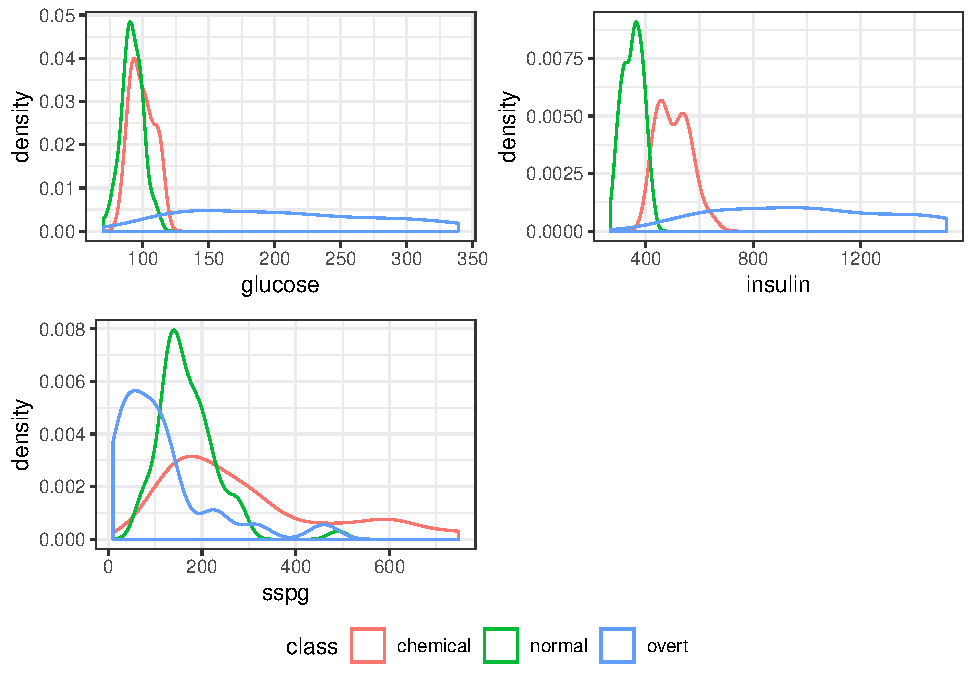
\includegraphics{Clase-4_files/figure-latex/unnamed-chunk-20-1.pdf}

\hypertarget{right}{}
\begin{verbatim}
plot(fit,plot.type="Shepard",plot.dim=c(1,2),sphere=TRUE,bubscale=0.1,col=1,
     label.conf=list(label=TRUE,pos=3,col=1,cex=0.8),
     shepard.x=NULL,identify=FALSE,
     type="p",pch=20,asp=1,col.hist=NULL)
\end{verbatim}

El ajuste casi perfecto entre disparidades y distancias se constata
también gráficamente usando el gráfico de Shepard.

\subsection{Desarrollo educativo de distintas zonas del
mundo}\label{desarrollo-educativo-de-distintas-zonas-del-mundo-8}

\hypertarget{left}{}
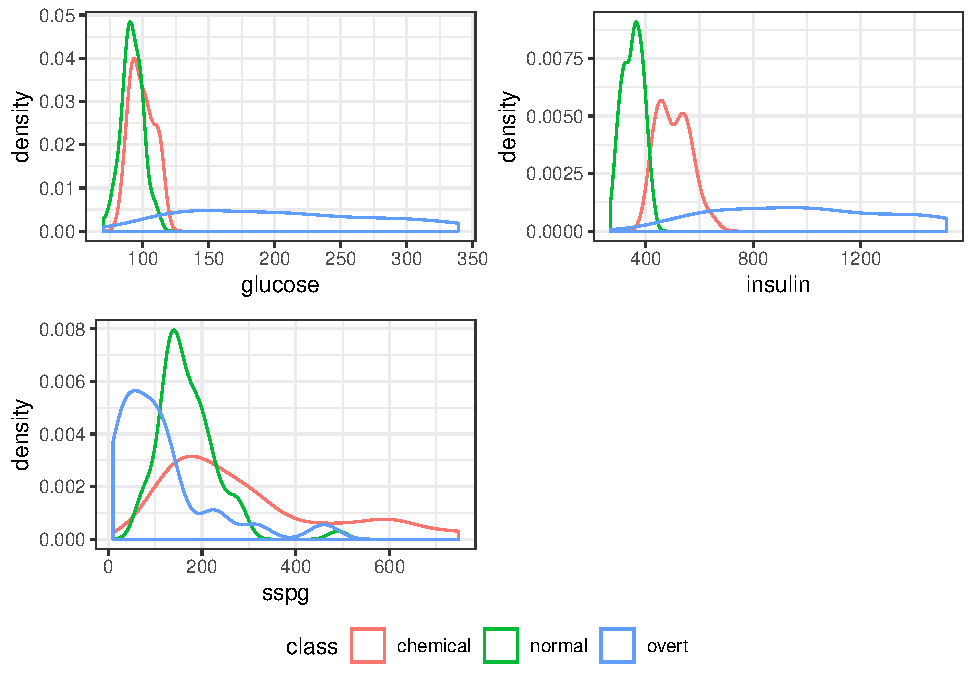
\includegraphics{Clase-4_files/figure-latex/unnamed-chunk-21-1.pdf}

\hypertarget{right}{}
Para corroborar que esta solución bidimensional es razonable. De no ser
así, si fuera necesario recurrir a cuatro o cinco dimensiones, el MDS no
ofrecería demasiada ayuda respecto al análisis de conglomerados, puesto
que el análisis gráfico de la solución sería complicado. Para corroborar
ensayamos distintas soluciones dimensionales (digamos de 1 a 7) y las
representamos en un gráfico las dimensiones en abscisas y el stress en
ordenadas. Si la solución bidimensional es válida, el stress debe caer
rápidamente hasta alcanzar esa dimensión, disminuyendo mucho menos en
dimensiones adicionales. La figura obtenida confirma que la solución
bidimensional es la adecuada.

\subsection{Desarrollo educativo de distintas zonas del
mundo}\label{desarrollo-educativo-de-distintas-zonas-del-mundo-9}

\begin{verbatim}
svec <- NULL
for (i in 1:7) {
  svec[i] <- mds(delta=datos, ndim = i, type = "ordinal")$stress
}

plot(seq(1:7),svec,type="overplotted", pch=16, ylab="Stress",xlab="Número de dimensiones")
\end{verbatim}

\subsection{Desarrollo educativo de distintas zonas del
mundo}\label{desarrollo-educativo-de-distintas-zonas-del-mundo-10}

Este código de R permite graficar la representación bidimensional de las
regiones usando el MSD.

\begin{verbatim}
plot(fit,plot.type="confplot",plot.dim=c(1,2),sphere=TRUE,bubscale=0.1,col=1,
     label.conf=list(label=TRUE,pos=3,col=1,cex=0.8),
     shepard.x=NULL,identify=FALSE,
     type="p",pch=20,asp=1,col.hist=NULL)
\end{verbatim}

\subsection{Desarrollo educativo de distintas zonas del
mundo}\label{desarrollo-educativo-de-distintas-zonas-del-mundo-11}

\hypertarget{left}{}
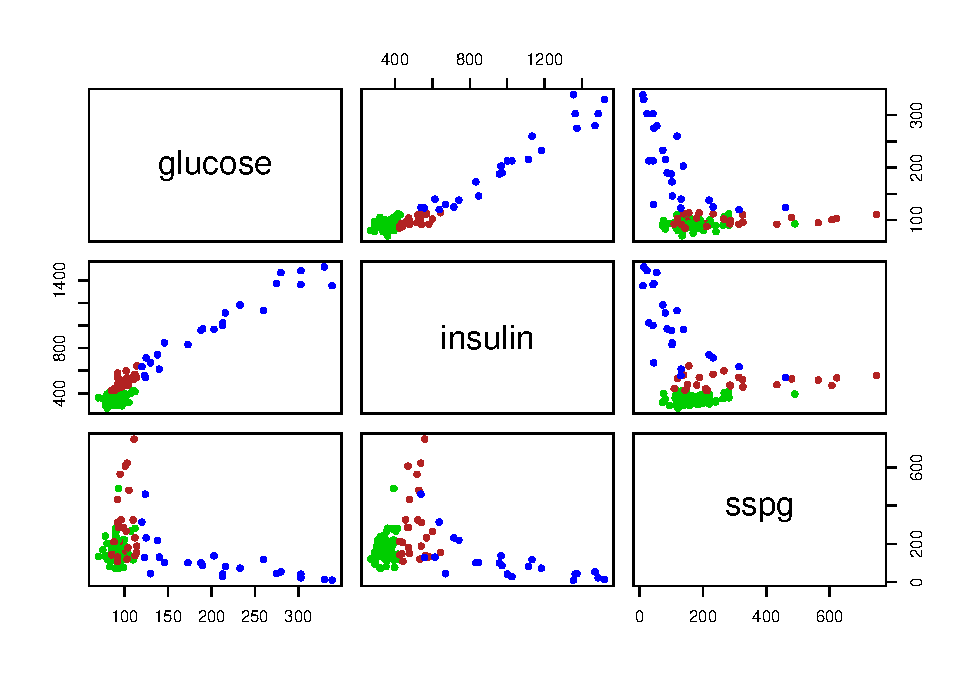
\includegraphics{Clase-4_files/figure-latex/unnamed-chunk-22-1.pdf}

\hypertarget{right}{}
La figura nos muestra que existen, al menos, tres grupos de regiones con
un desarrollo educativo muy diferenciado. Un grupo lo formarían América
del Norte (Z1), Asia / Oceanía (Z2) y Europa (Z3). Este grupo vendría
caracterizado por contener a los países con mayor desarrollo de sus
sistemas educativos. Téngase en cuenta que Z2 incluye solo a aquellos
países de Asia y Oceanía más avanzados, como son Japón, Nueva Zelanda o
Australia. Interpretamos que estos países son los más avanzados no solo
por el sentido común, difícil de aplicar en otro tipo de análisis, sino
porque son los más alejados de Z12, que, recordemos, incluía como
referencia a aquellos países menos adelantados.

\subsection{Desarrollo educativo de distintas zonas del
mundo}\label{desarrollo-educativo-de-distintas-zonas-del-mundo-12}

\hypertarget{left}{}
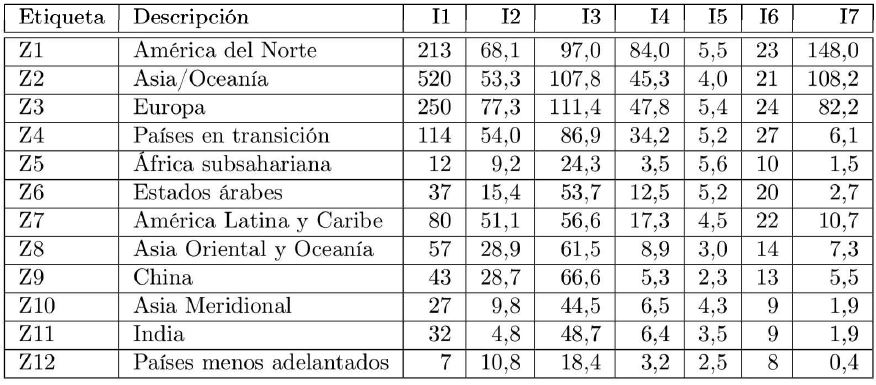
\includegraphics[width=1\linewidth]{images/cuadro}

\hypertarget{right}{}
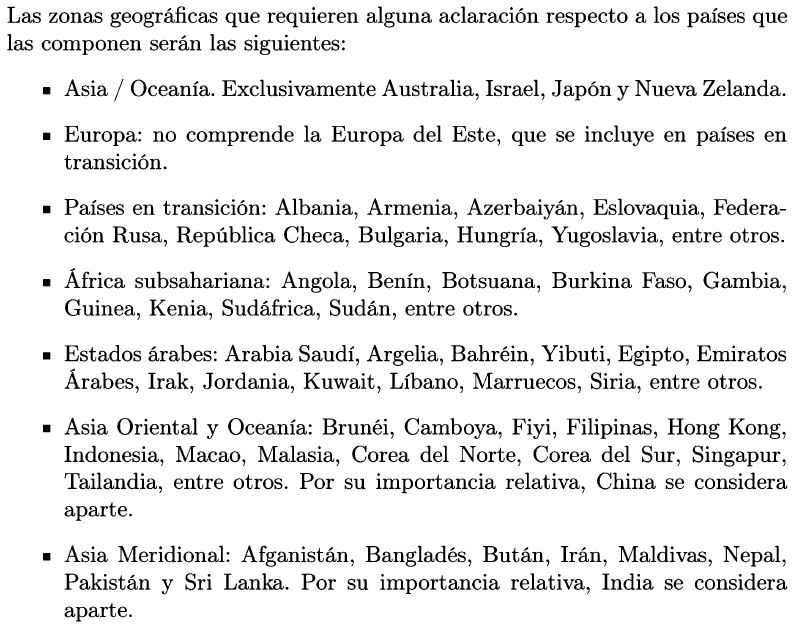
\includegraphics[width=1\linewidth]{images/geogra}

\subsection{Desarrollo educativo de distintas zonas del
mundo}\label{desarrollo-educativo-de-distintas-zonas-del-mundo-13}

\hypertarget{left}{}
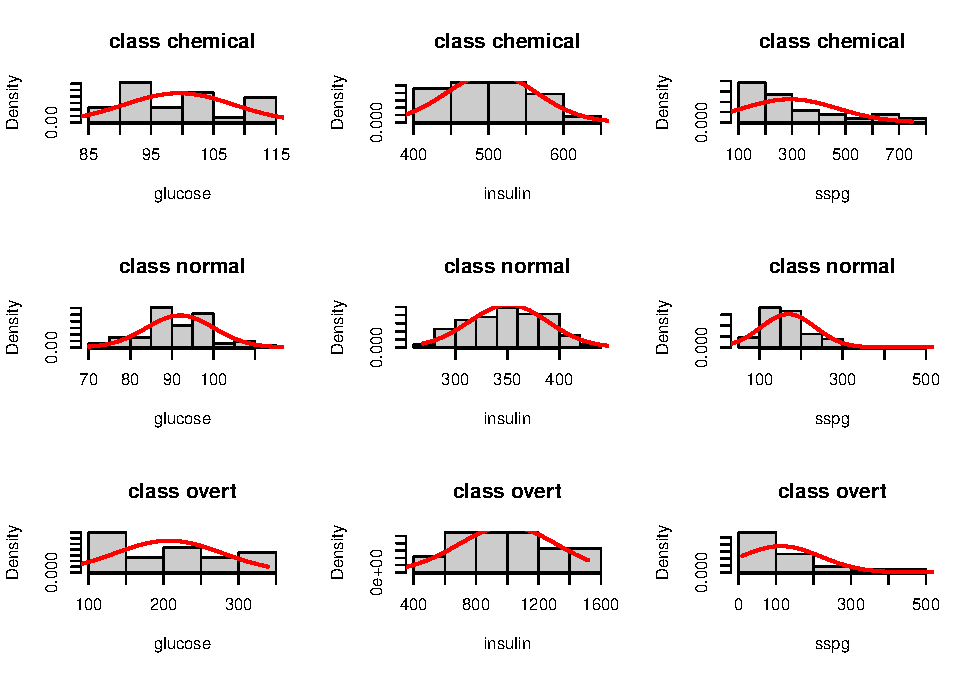
\includegraphics{Clase-4_files/figure-latex/unnamed-chunk-25-1.pdf}

\hypertarget{right}{}
Un grupo intermedio vendría formado por los países euroasiáticos en
transición (Z4), América Latina y el Caribe (Z7) y los Estados árabes
(Z6), que tendrían un desarrollo educativo intermedio entre los más
avanzados y los de menor desarrollo. Estos últimos serían los recogidos
en el mapa más cerca de Z12, es decir, Africa subsahariana, Asia
Oriental y Oceanía, Asia Meridional e India.

\subsection{Desarrollo educativo de distintas zonas del
mundo}\label{desarrollo-educativo-de-distintas-zonas-del-mundo-14}

\hypertarget{left}{}
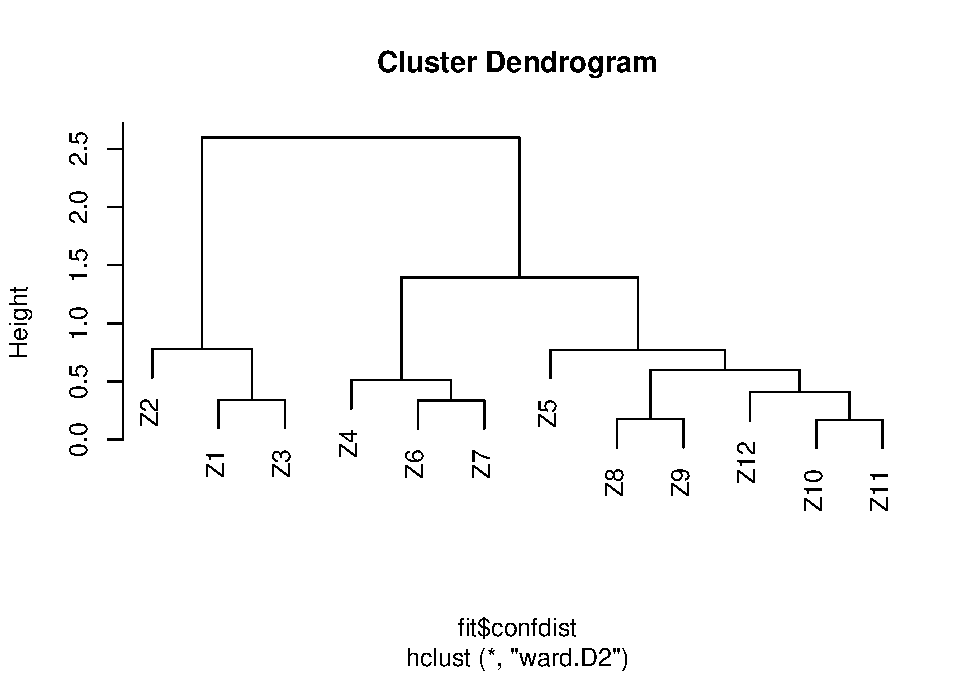
\includegraphics{Clase-4_files/figure-latex/unnamed-chunk-26-1.pdf}

\hypertarget{right}{}
Por qué considerar tres agregados y no más (o menos) en la
interpretación. Para ayudar en este tipo de análisis de los gráficos de
MDS, Kruskal y Wish (1978) recomiendan complementar esta técnica con
otras ya expuestas, como el análisis de conglomerados. Atendiendo a ese
dendograma, se han formado los grupos que, como se puede comprobar,
sirvió de base para la interpretación que expusimos con anterioridad.

\subsection{Ejemplo sobre psicología
clínica}\label{ejemplo-sobre-psicologuxeda-cluxednica}

El conjunto de datos proviene del área de psicología clínica. McNally et
al. (2015) recopilaron datos sobre los síntomas del TEPT (trastorno de
estrés postraumático) informados por los sobrevivientes del terremoto de
Wenchuan en China utilizando la lista de control civil (TEP-C; Weathers
et al., 1993). En total, hay 17 ítems de síntomas de trastorno de estrés
postraumático escalados en una escala de calificación de 5 puntos (1
\ldots{} ``para nada''; 5 \ldots{} ``extremadamente''). Estamos
interesados en representar asociaciones entre el TEPT. los síntomas.

\subsection{Ejemplo sobre psicología
clínica}\label{ejemplo-sobre-psicologuxeda-cluxednica-1}

\begin{verbatim}
library("MPsychoR")
data(Wenchuan)
head(Wenchuan)
\end{verbatim}

\begin{verbatim}
##   intrusion dreams flash upset physior avoidth avoidact amnesia lossint
## 1         2      2     2     2       3       2        3       2       3
## 2         2      2     2     3       3       3        3       2       3
## 3         2      4     4     4       3       3        3       5       4
## 4         2      1     2     2       1       1        2       2       2
## 5         2      2     2     2       2       2        2       2       3
## 6         4      3     2     2       2       2        3       3       2
##   distant numb future sleep anger concen hyper startle
## 1       2    2      1     3     4      3     4       2
## 2       3    2      2     3     3      2     3       3
## 3       3    2      3     4     4      4     3       4
## 4       1    1      2     2     1      2     3       3
## 5       2    2      2     3     2      3     2       3
## 6       2    2      3     2     3      2     3       2
\end{verbatim}

\subsection{Ejemplo sobre psicología
clínica}\label{ejemplo-sobre-psicologuxeda-cluxednica-2}

\hypertarget{left}{}
\begin{verbatim}

library("smacof")
Wdelta <- dist(t(Wenchuan)) ## Euclidean distances
fit.wenchuan1 <- mds(Wdelta, type = "ordinal") ## MDS fit
fit.wenchuan1
\end{verbatim}

\begin{verbatim}
## 
## Call:
## mds(delta = Wdelta, type = "ordinal")
## 
## Model: Symmetric SMACOF 
## Number of objects: 17 
## Stress-1 value: 0.133 
## Number of iterations: 35
\end{verbatim}

\hypertarget{right}{}
Primero, calculamos las similitudes derivadas utilizando la distancia
euclidiana, lo que resulta en una matriz de disimilitud simétrica de 17
× 17. Por un momento, consideremos un nivel de escala ordinal para las
diferencias de entrada y ajustemos un MDS ordinal bidimensional. El
ajuste de MDS da como resultado un valor de stress de 0.133. El valor
del stress en este ejemplo sugiere un ajuste regular del modelo.

\subsection{Ejemplo sobre psicología
clínica}\label{ejemplo-sobre-psicologuxeda-cluxednica-3}

\hypertarget{left}{}
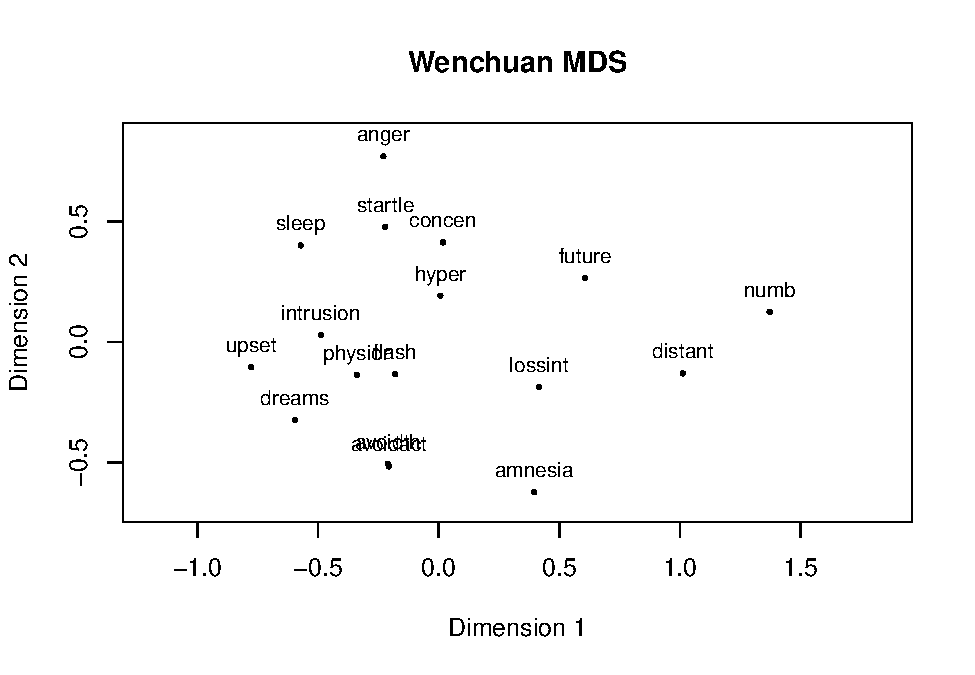
\includegraphics{Clase-4_files/figure-latex/unnamed-chunk-29-1.pdf}

\hypertarget{right}{}
\begin{verbatim}
plot(fit.wenchuan1, main = "Wenchuan MDS")
\end{verbatim}

El gráfico muestra cómo los síntomas de TEPT están relacionados entre
sí. Por ejemplo, vemos que ``evitar pensar o hablar sobre una
experiencia estresante del pasado o evitar tener sentimientos
relacionados con ella'' (avoidth) y ``evitar actividades o situaciones
porque le recordaron una experiencia estresante del pasado''(avoidact)
están virtualmente en el mismo lugar.

\subsection{Ejemplo sobre psicología
clínica}\label{ejemplo-sobre-psicologuxeda-cluxednica-4}

\hypertarget{left}{}
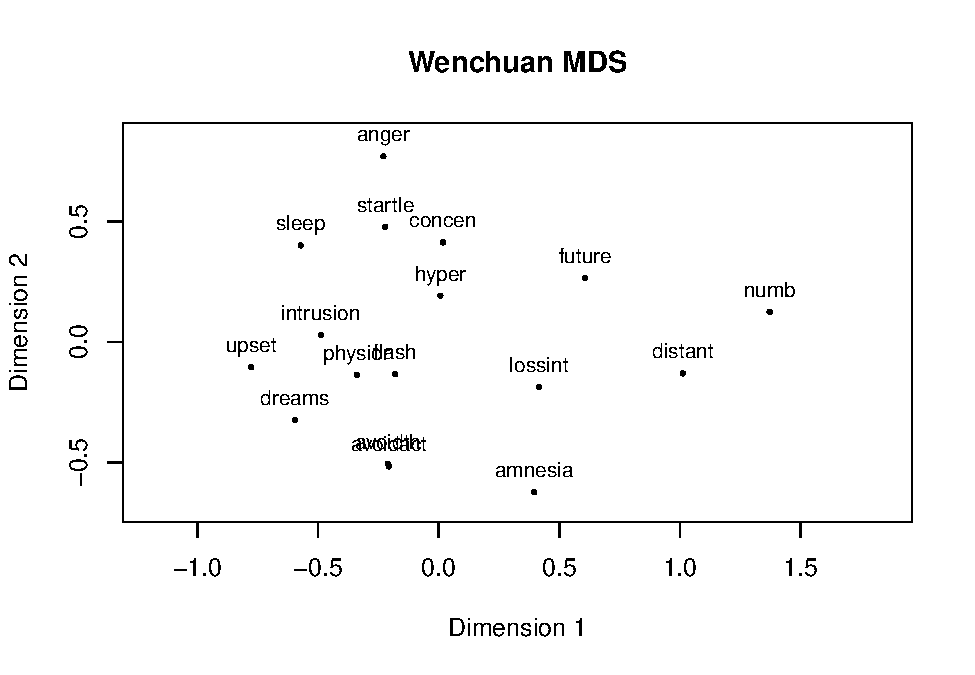
\includegraphics{Clase-4_files/figure-latex/unnamed-chunk-30-1.pdf}

\hypertarget{right}{}
También vemos que ``sentirse muy molesto cuando algo te recordó una
experiencia estresante del pasado?'' (upset) y ``sentirse emocionalmente
adormecido o ser incapaz de tener sentimientos amorosos para las
personas cercanas a usted'' (numb) son los puntos más lejanos en la
primera dimensión, mientras que ``problemas para recordar partes
importantes de una experiencia estresante del pasado'' (amnesia) y
``sentirse irritable o tener arrebatos de ira''(anger) son los puntos
extremos en la segunda dimensión. Estos pares de síntomas no están
relacionados entre sí.

\subsection{Ejemplo sobre psicología
clínica}\label{ejemplo-sobre-psicologuxeda-cluxednica-5}

Un error común es interpretar el stress de manera demasiado mecánica al
confiar solo en la tabla presentada anteriormente. Esto es problemático
debido a que la magnitud del stress depende de la cantidad de objetos
\(n\) (cuanto más grande es \(n\), mayor es el stress). En las
aplicaciones MDS modernas, \(n\) puede ser bastante grande. En lugar de
utilizar estas reglas generales, podemos considerar enfoques de
simulación. Un enfoque antiguo (Spence y Ogilvie, 1973) es simular
diferencias aleatorias para \(n\) y \(p\) fijas y ajustar el modelo MDS
correspondiente en estas matrices. Esto conduce a
\texttt{random\ stress\ norms}.

\subsection{Ejemplo sobre psicología
clínica}\label{ejemplo-sobre-psicologuxeda-cluxednica-6}

\hypertarget{left}{}
\begin{verbatim}
set.seed(123)
rsvec <- randomstress(n = attr(Wdelta, "Size"), ndim = 2,
                      nrep = 500, type = "ordinal")
mean(rsvec)
mean(rsvec) - 2*sd(rsvec)
\end{verbatim}

\begin{verbatim}
## [1] 0.2770934
\end{verbatim}

\begin{verbatim}
## [1] 0.2548536
\end{verbatim}

\hypertarget{right}{}
El llamado \texttt{randomstress} da 500 valores de stress aleatorios.
Estos estándares de stress representan un punto de referencia de ``mal
ajuste''. Nuestra solución debe estar claramente por debajo del stress
aleatorio promedio. A menudo, en la literatura, los valores de stress
observados se consideran ``significativos'' si son más pequeños que el
límite de estrés aleatorio inferior 2 × sd, que es claramente el caso en
nuestro ejemplo (el estrés fue 0.133).

\subsection{Ejemplo sobre psicología
clínica}\label{ejemplo-sobre-psicologuxeda-cluxednica-7}

\hypertarget{left}{}
\begin{verbatim}
set.seed(123)
permmds <- permtest(fit.wenchuan1, data = Wenchuan,
                    method.dat = "euclidean", nrep = 500,
                    verbose = FALSE)
permmds
\end{verbatim}

\begin{verbatim}
## 
## Call: permtest.smacof(object = fit.wenchuan1, data = Wenchuan, method.dat = "euclidean", 
##     nrep = 500, verbose = FALSE)
## 
## SMACOF Permutation Test
## Number of objects: 17 
## Number of replications (permutations): 500 
## 
## Observed stress value: 0.133 
## p-value: <0.001
\end{verbatim}

\hypertarget{right}{}
Un enfoque más preciso es utilizar una prueba de permutación como se
describe en Mair et al. (2016). Para las diferencias similares, vuelve a
muestrear los datos originales, y para cada matriz de desigualdad
resultante, se lleva a cabo un ajuste MDS. Esto proporciona una
distribución del estrés bajo el \(H_0\): ``el stress / configuración se
obtiene de una permutación aleatoria de diferencias''. Como \(p<0.05\),
rechazamos el \(H_0\) y concluimos que el stress / configuración se
obtiene de algo distinto a una permutación aleatoria de diferencias.

\subsection{Ejemplo sobre psicología
clínica}\label{ejemplo-sobre-psicologuxeda-cluxednica-8}

\hypertarget{left}{}
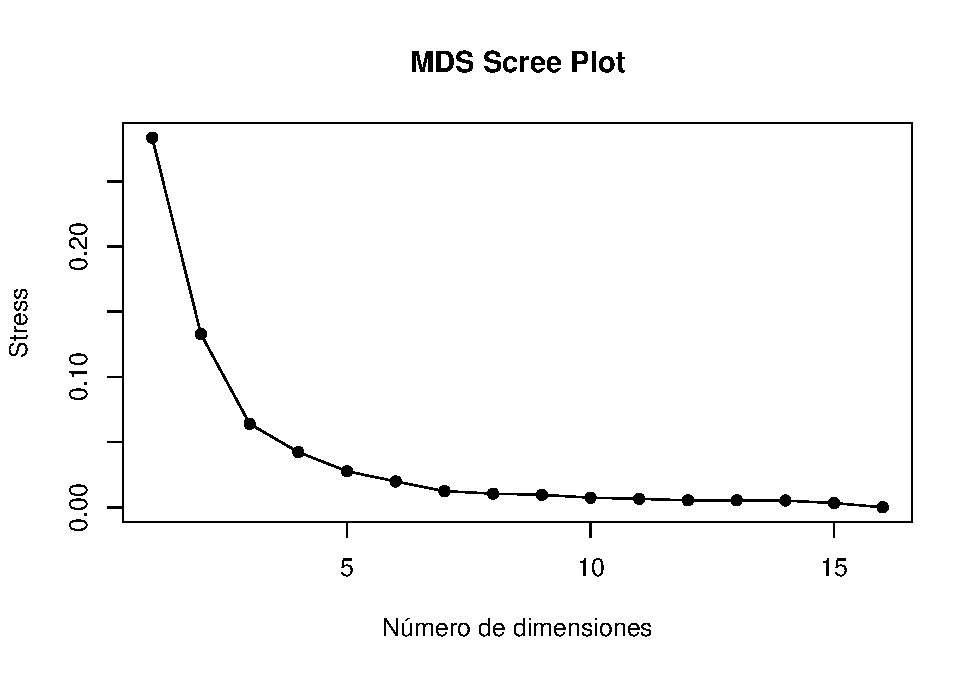
\includegraphics{Clase-4_files/figure-latex/unnamed-chunk-33-1.pdf}

\hypertarget{right}{}
\begin{verbatim}
n <- attr(Wdelta, "Size")
svec <- NULL
for (i in 1:(n-1)) {
  svec[i] <- mds(Wdelta, ndim = i, type = "ordinal")$stress
}

plot(seq(1:(n-1)),svec,type="overplotted", pch=16, ylab="Stress",
xlab="Número de dimensiones", main="MDS Scree Plot")
\end{verbatim}

Basándonos únicamente en el scree plot, probablemente elegiríamos una
solución 3D, pero el stress de la solución 2D tampoco es demasiado malo,
como lo juzgan las \texttt{random\ stress\ norms}, los resultados de las
pruebas de permutación y la tabla de referencia de los valores de stress
(considerados aquí como n = 17 es bastante pequeño).

\subsection{Ejemplo sobre psicología
clínica}\label{ejemplo-sobre-psicologuxeda-cluxednica-9}

Se sabe que la función de objetivo de estrés es irregular. Por lo tanto,
puede suceder fácilmente que terminemos en un mínimo local (es decir, no
obtenemos la mejor solución posible). Donde el algoritmo termina al
final depende de donde comienza. De forma predeterminada, las funciones
en el paquete \texttt{smacof} utilizan una solución de escala clásica
(Torgerson, 1952) como configuración inicial. Esta no es necesariamente
la mejor opción. El problema mínimo local que incluye una búsqueda
sistemática de soluciones iniciales se describe en detalle en Borg y
Mair (2017). Aquí utilizamos una estrategia ad hoc simple al probar
diferentes inicios aleatorios y verificar si la mejor solución de inicio
aleatorio conduce a un valor de estrés más bajo que la configuración
predeterminada.

\subsection{Ejemplo sobre psicología
clínica}\label{ejemplo-sobre-psicologuxeda-cluxednica-10}

\hypertarget{left}{}
\begin{verbatim}
## [1] 0.1327943
\end{verbatim}

\begin{verbatim}
## [1] 0.1328058
\end{verbatim}

\hypertarget{right}{}
A continuación examinamos 100 inicios aleatorios y extraemos los valores
de estrés. Vemos que un inicio aleatorio en particular proporcionó un
stress ligeramente mejor que nuestra solución original. Dado que la
diferencia de estrés es tan mínima, podemos elegir cualquiera de las dos
soluciones.

\subsection{Ejemplo sobre psicología
clínica}\label{ejemplo-sobre-psicologuxeda-cluxednica-11}

\begin{verbatim}
set.seed(123)
fit.wenchuan <- NULL ## 100 random starts
for(i in 1:100) {
  fit.wenchuan[[i]] <- mds(Wdelta, type = "ordinal",
                           init = "random")
}
## extract the best solution
ind <- which.min(sapply(fit.wenchuan,
                        function(x) x$stress))
fit.wenchuan2 <- fit.wenchuan[[ind]]
fit.wenchuan2$stress ## lowest stress (random start)

fit.wenchuan1$stress ## stress (classical scaling start)
\end{verbatim}

\subsection{Ejemplo sobre psicología
clínica}\label{ejemplo-sobre-psicologuxeda-cluxednica-12}

\hypertarget{left}{}
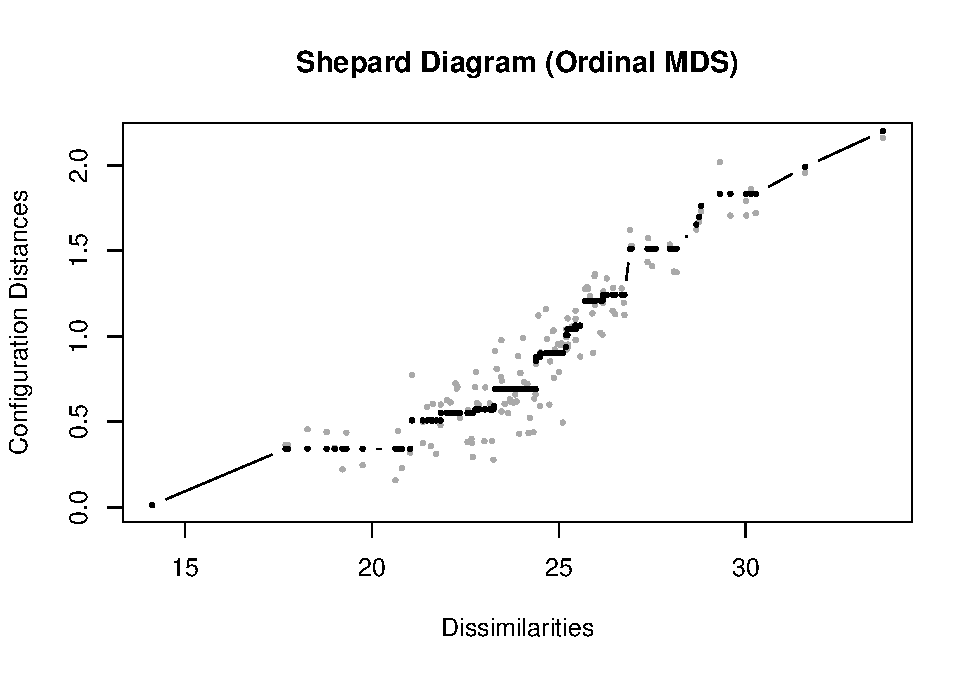
\includegraphics{Clase-4_files/figure-latex/unnamed-chunk-35-1.pdf}

\hypertarget{right}{}
\begin{verbatim}
plot(fit.wenchuan2, plot.type = "Shepard",
     main = "Shepard Diagram (Ordinal MDS)")
\end{verbatim}

Vemos varios puntos grises alejados de la recta, lo cual explica porque
el valor de stress no está en el rango de bueno a excelente.

\subsection{Ejemplo sobre psicología
clínica}\label{ejemplo-sobre-psicologuxeda-cluxednica-13}

\hypertarget{left}{}
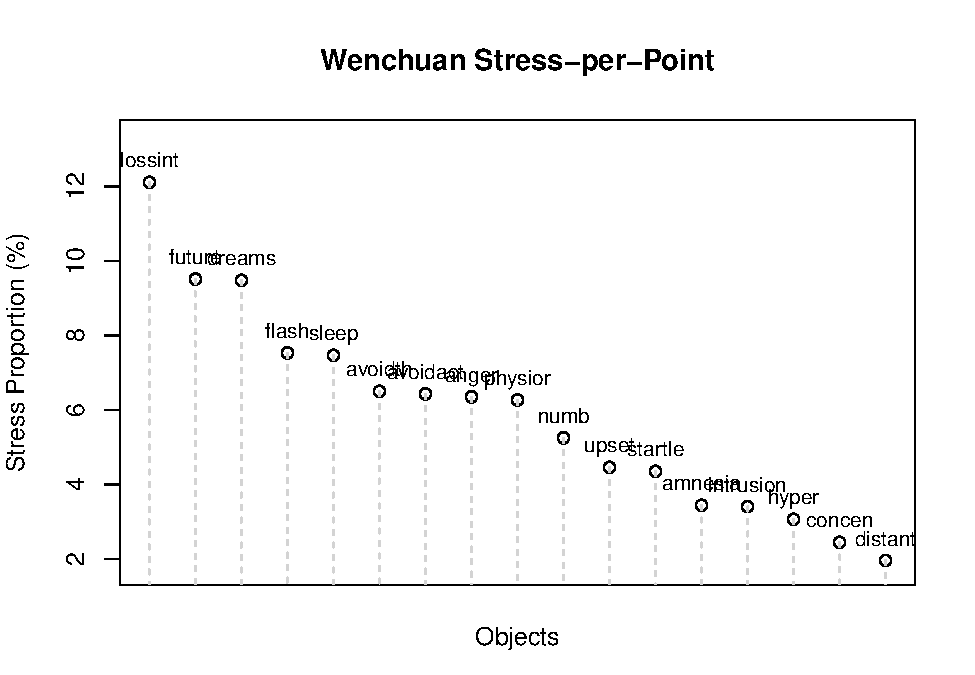
\includegraphics{Clase-4_files/figure-latex/unnamed-chunk-36-1.pdf}

\hypertarget{right}{}
\begin{verbatim}
plot(fit.wenchuan2, plot.type = "stressplot",
     main = "Wenchuan Stress-per-Point")
\end{verbatim}

La contribución de cada objeto al stress total se puede calcular
fácilmente. Los valores resultantes, que normalmente se informan como
porcentajes, se denominan stress por punto (SPP). Podemos pensar en
puntos con una alta contribución de SPP de manera similar a los valores
atípicos influyentes en la regresión. En nuestro ejemplo, vemos que la
``pérdida de interés en actividades que solía disfrutar'' (lossint)
proporciona una contribución de estrés bastante alta del 12.11\%.


\end{document}
